%%% File-Information {{{
%%% Filename: Korrekturen.tex
%%% }}}
%%%%%%%%%%%%%%%%%%%%%%%%%%%%%%%%%%%%%%%%%%%%%%%%%%%%%%%%%%%%%%%%%%%%%%%%%%%%%%%%
%%% main document {{{

\documentclass[
a4paper,     %% defines the paper size: a4paper (default), a5paper, letterpaper, ...
% landscape,   %% sets the orientation to landscape
% twoside,     %% changes to a two-page-layout (alternatively: oneside)
% twocolumn,   %% changes to a two-column-layout
headsepline, %% add a horizontal line below the column title
footsepline, %% add a horizontal line above the page footer
titlepage,   %% only the titlepage (using titlepage-environment) appears on the first page (alternatively: notitlepage)
halfparskip,     %% insert an empty line between two paragraphs (alternatively: halfparskip, ...)
% leqno,       %% equation numbers left (instead of right)
% fleqn,       %% equation left-justified (instead of centered)
% tablecaptionabove, %% captions of tables are above the tables (alternatively: tablecaptionbelow)
%draft,       %% produce only a draft version (mark lines that need manual edition and don't show graphics)
% 10pt         %% set default font size to 10 point
12pt,         %% set default font size to 11 point
DIV16
]{scrartcl}  %% article, see KOMA documentation (scrguide.dvi)

%%%%%%%%%%%%%%%%%%%%%%%%%%%%%%%%%%%%%%%%%%%%%%%%%%%%%%%%%%%%%%%%%%%%%%%%%%%%%%%%
%%%
%%% packages
%%%

\usepackage{pstricks}
\usepackage{vaucanson-g}

%%%
%%% encoding and language set
%%%

%%% ngerman: language set to new-german
\usepackage{ngerman}

%%% inputenc: coding of german special characters
\usepackage[latin1]{inputenc}

%%% fontenc, ae, aecompl: coding of characters in PDF documents
\usepackage[T1]{fontenc}
\usepackage{ae,aecompl}

%%%
%%% technical packages
%%%

%%% amsmath, amssymb, amstext: support for mathematics
\usepackage{amsmath,amssymb,amstext}

%%% psfrag: replace PostScript fonts
\usepackage{psfrag}

%%% listings: include programming code
\usepackage{listings}
\usepackage{moreverb}

%%% units: technical units
\usepackage{units}

%%% color: support for ... colors, yes!
\usepackage{color}

%%% graphs and automata (has to be loaded _before_ ngerman)
\usepackage{pstricks}
\usepackage{vaucanson-g}

%%% table-stuff
\usepackage{booktabs}
\usepackage{array}
\usepackage{multirow}

\newcolumntype{N}{>{\bfseries\scriptsize}l}
\newcolumntype{V}[1]{%
	>{\bfseries\scriptsize\raggedright\hspace{0pt}}p{#1}%
}

%%% some color-definitions (see http://texnik.de/listings/listing0.pdf)
\definecolor{hellgelb}{rgb}{1,1,0.8}
\definecolor{hellgrau}{rgb}{0.9,0.9,0.9}
\definecolor{colKeys}{rgb}{0,0,1}
\definecolor{colIdentifier}{rgb}{0,0,0}
\definecolor{colComments}{rgb}{1,0,0}
\definecolor{colString}{rgb}{0,0.5,0}

%%% configuration of the listings-package
\lstset{%
	float=hbp,%
	basicstyle=\ttfamily\small, %
	identifierstyle=\color{colIdentifier}, %
	keywordstyle=\color{colKeys}, %
	stringstyle=\color{colString}, %
	commentstyle=\color{colComments}, %
	columns=flexible, %
	tabsize=4, %
	frame=tb, %
	extendedchars=true, %
	showspaces=false, %
	showstringspaces=false, % 
	numbers=left, %
	numberstyle=\tiny, %
	breaklines=true, %
	backgroundcolor=\color{hellgrau}, %
	breakautoindent=true, %
	captionpos=b%
}

%%%
%%% layout
%%%

%%% scrpage2: KOMA heading and footer
%%% Note: if you don't use this package, please remove 
%%%       \pagestyle{scrheadings} and corresponding settings
%%%       below too.
\usepackage{scrpage2}

% EM unterstrichen darstellen
%\usepackage{ulem}

% Schrift fuer Captions verkleinern
%\setkomafont{captionlabel}{\scriptsize}
%\setkomafont{caption}{\usekomafont{captionlabel}}

% Float
\usepackage{float}


%%%
%%% PDF
%%%

\newif\ifpdf
  \ifx\pdfoutput\undefined
     \pdffalse
  \else
     \pdfoutput=1
     \pdftrue
  \fi

%%% Should be LAST usepackage-call!
%%% For docu on that, see reference on package ``hyperref''
\ifpdf{%   (definitions for using pdflatex instead of latex)

	%%% for screen (PDF), we use sans-serif-fonts
	%\usepackage{mathpazo}
	\usepackage{mathptmx}
	\usepackage[scaled=.95]{helvet}
	\usepackage{courier}	
	\renewcommand{\familydefault}{\sfdefault}
	\usepackage[sf]{titlesec}

  %%% graphicx: support for graphics
  \usepackage[pdftex]{graphicx}
 
  \pdfcompresslevel=9

  %%% hyperref (hyperlinks in PDF): for more options or more detailed
  %%%          explanations, see the documentation of the hyperref-package
  \usepackage[%
    %%% general options
    pdftex=true,      %% sets up hyperref for use with the pdftex program
    %plainpages=false, %% set it to false, if pdflatex complains: ``destination with same identifier already exists''
    %
    %%% extension options
    backref=section,   %% if true, adds a backlink text to the end of each item in the bibliography
    pagebackref=false, %% if true, creates backward references as a list of page numbers in the bibliography
    colorlinks=true,   %% turn on colored links (true is better for on-screen reading, false is better for printout versions)
    %
    %%% PDF-specific display options
    bookmarks=true,          %% if true, generate PDF bookmarks (requires two passes of pdflatex)
    bookmarksopen=false,     %% if true, show all PDF bookmarks expanded
    bookmarksnumbered=false, %% if true, add the section numbers to the bookmarks
    %pdfstartpage={1},        %% determines, on which page the PDF file is opened
    pdfpagemode=None,	       %% None, UseOutlines (=show bookmarks), UseThumbs (show thumbnails), FullScreen
    breaklinks=true         
  ]{hyperref}


  %%% provide all graphics (also) in this format, so you don't have
  %%% to add the file extensions to the \includegraphics-command
  %%% and/or you don't have to distinguish between generating
  %%% dvi/ps (through latex) and pdf (through pdflatex)
  \DeclareGraphicsExtensions{.pdf}
  \graphicspath{{./images}}

\else    %(definitions for using latex instead of pdflatex)

  \usepackage[dvips]{graphicx}

  \DeclareGraphicsExtensions{.eps}
  \graphicspath{{./images}}  

  \usepackage[%
    dvips,            %% sets up hyperref for use with the dvips driver
    colorlinks=false, %% better for printout version; almost every hyperref-extension is eliminated by using dvips
    breaklinks=true 
  ]{hyperref}

\fi %ifpdf

%%% sets the PDF-Information options
%%% (see fields in Acrobat Reader: ``File -> Document properties -> Summary'')
%%% Note: this method is better than as options of the hyperref-package (options are expanded correctly)
\hypersetup{
  pdftitle={<Aufgaben-Titel>}, %%
  pdfauthor={Christoph Eck <ceck@fh-konstanz.de>, Jan Tammen <foobar@fh-konstanz.de>}, %%
  pdfsubject={Objektorientierte Programmierung, �bungsaufgabe 3: Teil 2}, %%
  pdfcreator={Jan Tammen <foobar@fh-konstanz.de>}, %% 
  pdfproducer={}, %%
  pdfkeywords={} %%
}


%%%%%%%%%%%%%%%%%%%%%%%%%%%%%%%%%%%%%%%%%%%%%%%%%%%%%%%%%%%%%%%%%%%%%%%%%%%%%%%%
%%%
%%% user defined commands
%%%

%%% \mygraphics{}{}{}
%% usage:   \mygraphics{width}{filename_without_extension}{caption}
%% example: \mygraphics{0.7\textwidth}{rolling_grandma}{This is my grandmother on inlinescates}
%% requires: package graphicx
%% provides: including centered pictures/graphics with a boldfaced caption below
%% 
\newcommand{\mygraphics}[3]{
  \begin{center}
    \includegraphics[width=#1, keepaspectratio=true]{#2} \\
    \textbf{#3}
  \end{center}
}

%%%%%%%%%%%%%%%%%%%%%%%%%%%%%%%%%%%%%%%%%%%%%%%%%%%%%%%%%%%%%%%%%%%%%%%%%%%%%%%%
%%%
%%% define the titlepage
%%%

% \subject{}   %% subject which appears above titlehead
% \titlehead{} %% special heading for the titlepage

%%% title
\title{Pizza-Service}

\subject{Objektorientierte Programmierung, �bungsaufgabe 3}

%%% author(s)
\author{Christoph Eck \href{mailto:ceck@fh-konstanz.de}{<ceck@fh-konstanz.de>}
					\and{%
						Jan Tammen \href{mailto:foobar@fh-konstanz.de}{<foobar@fh-konstanz.de>}
					}%
				}%

\publishers{Teil 2}

\date{\today}

% \thanks{} %% use it instead of footnotes (only on titlepage)

% \dedication{} %% generates a dedication-page after titlepage

%%%%%%%%%%%%%%%%%%%%%%%%%%%%%%%%%%%%%%%%%%%%%%%%%%%%%%%%%%%%%%%%%%%%%%%%%%%%%%%%
%%%
%%% set heading and footer
%%%

%%% scrheadings default: 
%%%      footer - middle: page number
\pagestyle{scrheadings}

%%% user specific
%%% usage:
%%% \position[heading/footer for the titlepage]{heading/footer for the rest of the document}

%%% heading - left
% \ihead[]{}

%%% heading - center
% \chead[]{}

%%% heading - right
% \ohead[]{}

%%% footer - left
% \ifoot[]{}

%%% footer - center
% \cfoot[]{}

%%% footer - right
% \ofoot[]{}



%%%%%%%%%%%%%%%%%%%%%%%%%%%%%%%%%%%%%%%%%%%%%%%%%%%%%%%%%%%%%%%%%%%%%%%%%%%%%%%%
%%%
%%% begin document
%%%

\begin{document}

% \pagenumbering{roman} %% small roman page numbers

%%% include the title
%\thispagestyle{empty}  %% no header/footer (only) on this page
\maketitle

%%% start a new page and display the table of contents
\newpage
%\tableofcontents

%%% start a new page and display the list of figures
%\newpage
%\listoffigures

%%% start a new page and display the list of tables
% \newpage
% \listoftables

%%% display the main document on a new page 
%\newpage

% \pagenumbering{arabic} %% normal page numbers (include it, if roman was used above)

%%%%%%%%%%%%%%%%%%%%%%%%%%%%%%%%%%%%%%%%%%%%%%%%%%%%%%%%%%%%%%%%%%%%%%%%%%%%%%%%
%%%
%%% begin main document
%%% structure: \section \subsection \subsubsection \paragraph \subparagraph
%%%

\section{UML Sequenzdiagramm}
\begin{figure}[H]
	\centering
		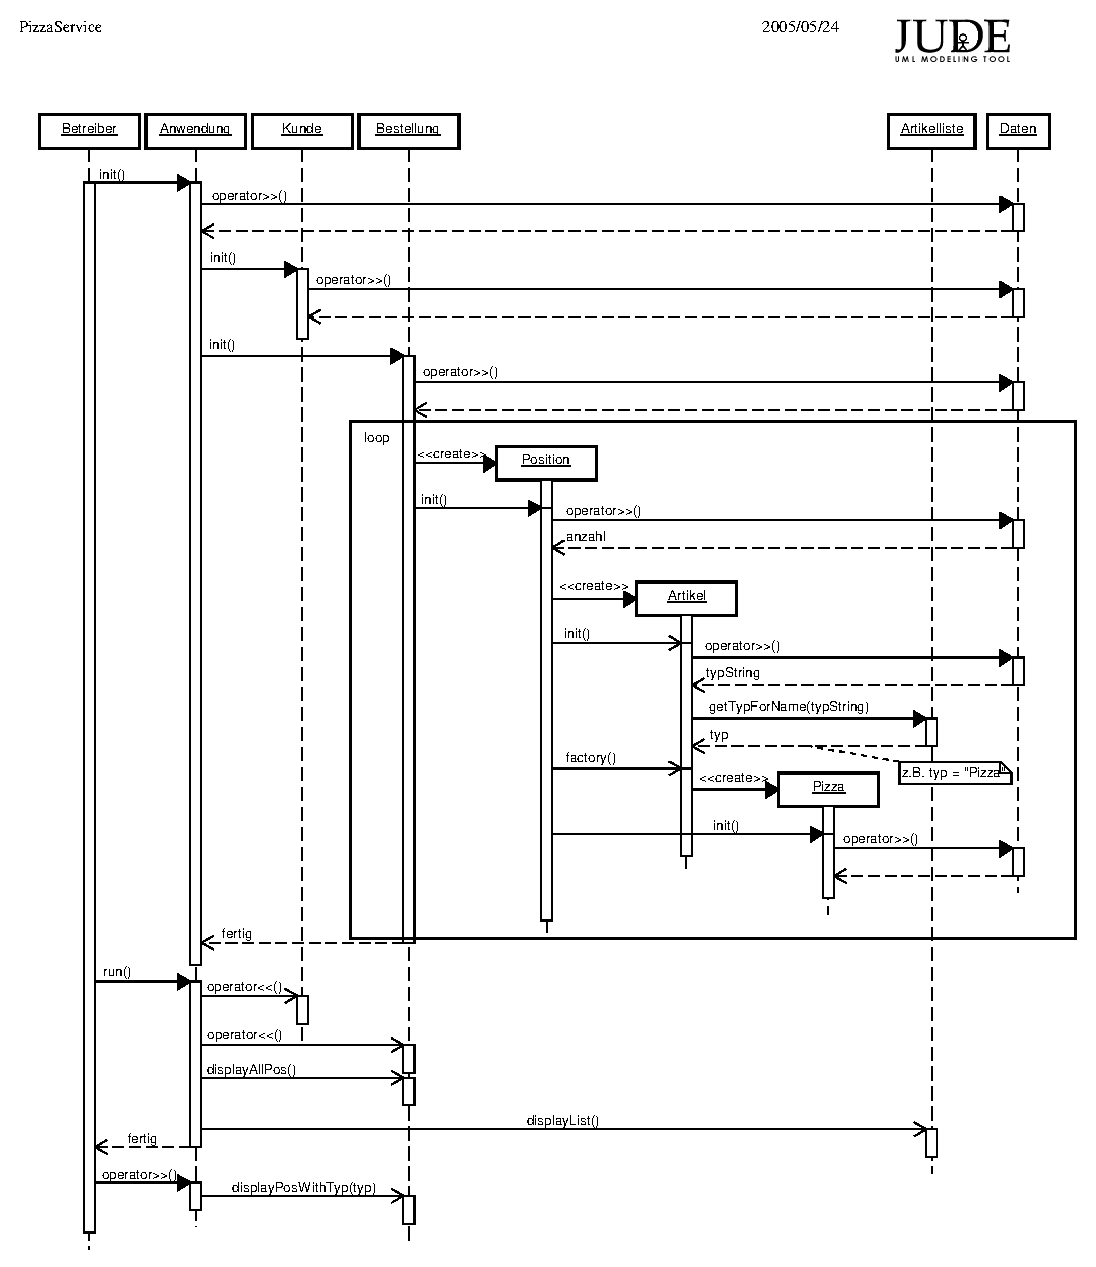
\includegraphics[width=1.0\textwidth,bb=45 196 554 760, clip]{images/sequenz_init.eps}
	\caption{UML Sequenzdiagramm}
	\label{fig:sequenz_init}
\end{figure}

\section{Erg�nzungen und Korrekturen}
Gegen�ber dem Originalkonzept wurden einige Erg�nzungen gemacht, welche im folgenden aufgef�hrt sind.

\subsection{Klasse Artikel}
Die Klasse \texttt{Artikel} ist nicht mehr als abstrakt deklariert, da sie nun gleichzeitig eine 
Fabrik-Methode \texttt{factory()} zur Verf�gung stellt, mit welcher die konkreten \texttt{Artikel}-Objekte
erstellt werden k�nnen.
\subsubsection{Klasse Getraenk}
Da die abstrakte Klasse \texttt{Getraenk} keinerlei Funktion beinhaltete (\texttt{Bier} und \texttt{Limo}
haben keine gemeinsamen Attribute und/oder Methoden, daher macht es keinen Sinn, sie von einer "`k�nstlichen"'
Eltern-Klasse abzuleiten), wurde sie komplett entfernt.

\subsection{Klasse Artikelliste}
�ber die neu hinzugef�gte Klasse \texttt{Artikelliste} werden alle verf�gbaren Artikel verwaltet -- d.h.
hier findet die Zuordnung zwischen dem Namen eines Artikels (z.B. "`Pizza"') und der internen ID (\texttt{enum Artikeltyp}) statt.
So k�nnen z.B. weitere Artikel durch Erg�nzung der Aufz�hlung \texttt{Artikeltyp} sowie Einf�gen in die Liste
\texttt{mListe} hinzugef�gt werden.

\subsection{Klasse Daten}
Diese ebenfalls zus�tzliche Klasse erm�glicht den einzelnen Objekten den Zugriff auf die Datendatei, damit sie
jeweils ihre eigenen Attribute initialisieren k�nnen.
Dabei wurde das Singleton-Muster angewandt, um sicherzustellen, dass es lediglich einen globalen Dateizugriff
gibt.

\subsection{Klasse Anwendung}
Die Klasse \texttt{Anwendung} aus dem Originalkonzept verf�gt nun �ber folgende Methoden:

\begin{itemize}
	\item \texttt{init()}: deligiert das Einlesen der Daten an die Objektattribute \texttt{mKunde} und \texttt{mBestellung}
	\item \texttt{run()}: f�hrt die eigentliche Anwendung aus, startet den Dialog mit dem Benutzer und gibt die Daten aus.
\end{itemize}
%%%
%%% end main document
%%%
%%%%%%%%%%%%%%%%%%%%%%%%%%%%%%%%%%%%%%%%%%%%%%%%%%%%%%%%%%%%%%%%%%%%%%%%%%%%%%%%

%\appendix  %% include it, if something (bibliography, index, ...) follows below

%%%%%%%%%%%%%%%%%%%%%%%%%%%%%%%%%%%%%%%%%%%%%%%%%%%%%%%%%%%%%%%%%%%%%%%%%%%%%%%%
%%%
%%% bibliography
%%%
%%% available styles: abbrv, acm, alpha, apalike, ieeetr, plain, siam, unsrt
%%%
% \bibliographystyle{plain}

%%% name of the bibliography file without .bib
%%% e.g.: literatur.bib -> \bibliography{literatur}
% \bibliography{FIXXME}

\end{document}
%%% }}}
%%% END OF FILE
%%%%%%%%%%%%%%%%%%%%%%%%%%%%%%%%%%%%%%%%%%%%%%%%%%%%%%%%%%%%%%%%%%%%%%%%%%%%%%%%
%%% Notice!
%%% This file uses the outline-mode of emacs and the foldmethod of Vim.
%%% Press 'zi' to unfold the file in Vim.
%%% See ':help folding' for more information.
%%%%%%%%%%%%%%%%%%%%%%%%%%%%%%%%%%%%%%%%%%%%%%%%%%%%%%%%%%%%%%%%%%%%%%%%%%%%%%%%
%% Local Variables:
%% mode: outline-minor
%% OPToutline-regexp: "%% .*"
%% OPTeval: (hide-body)
%% emerge-set-combine-versions-template: "%a\n%b\n"
%% End:
%% vim:foldmethod=marker